   \subsection{A new version of multi-grid algorithm}
   If we look at the previous section, we see that at some point, even if we increase the number of cycles we do, we reach a lower bound (which depends on the topology and the problem considered) on the accuracy we can achieve (for example on Figure~\ref{fig.first_tests}, it is around $10^{-15}$). This bound comes from the internal limitations of the \texttt{double} type.
   Indeed, a double uses 8 bytes (52 bits for the mantissa, 11 for the exponent and 1 bit for the sign). This representation does not allow a full description of all rational numbers (for example between $2^{52}$ and $2^{53}$ only integers can be represented).
   If we increase the number of bits of the mantissa or the exponent we can describe more and more numbers. In the other way, if we reduce it, we lose accuracy for numbers that are not representable. Considering our algorithm, what if we only want
   a precision of only $10^{-3}$ ? We don't need the 64 bits of a \texttt{double}, to reach it, a smaller number is enough. The advantage of using less bits for the floating point numbers is a faster and energy-saving computation. Thus it is important
   to study the impact of using a representation with smaller mantissa.
   
   To realize these experiments, we use two modified versions of the original algorithm. We modify the function that does the relaxation step (remember it is the costly part of the whole algorithm).
   In this function we can find different internal variables that are originally of type \texttt{double}: 5 arrays and 8 scalars. We will denote by \emph{AMG} this original algorithm. The first version, \emph{AMGfloat}, changes the type of these 13 variables from \texttt{double*} or \texttt{double}
   to \texttt{float*} or \texttt{float}. For the second version, we use the library MPFR~\cite{MPFR,MPFR_link} that introduces a type \texttt{mpfr\_t}. This type has a parameter which is the number of bits in the mantissa of the variable.
   Every computation is done exactly, meaning that it is first computed as if there was an infinite number of bits, then rounded to a number using exactly the number of bits set as parameter. We build the second version, \emph{AMGmpfr(b)}: \emph{AMGmpfr(b)} is the algorithm \emph{AMG} where the 8 scalar variables of the relaxation function are replaced
   by \texttt{mpfr\_t} variables, all using the same number of $b$ bits for the mantissa. In terms of arithmetic precision, \emph{AMG} behaves similarly to \emph{AMGmpfr(53)} and \emph{AMGfloat} to \emph{AMGmpfr(24)}. There can be small differences
   due to the rounding method used.
   
   The Figure~\ref{fig.bits_accuracy} represent the accuracy we reach using either \emph{AMGmpfr(8)}, \emph{AMGmpfr(16)}, \emph{AMGfloat}, \emph{AMGmpfr(32)} or \emph{AMGmpfr(64)}. The problem used is \textsc{Unstructured-Anisotropy}, with 2x2x2 processor topology and 20x20x20 matrix size.
   What we actually see on this figure is the threshold reachable depending on the number of bits used. However, until this threshold is reach, the accuracy obtained using any number of bits is the same. This means that, for example,
   while the accuracy of the solution is below the threshold using 32 bits, using 32 or any greater number of bits to do the computations will result in the same final accuracy. However, we expect that using only the necessary $32$ bits is 
   more efficient in terms of time, space and energy.
   
   \begin{figure} \centering
    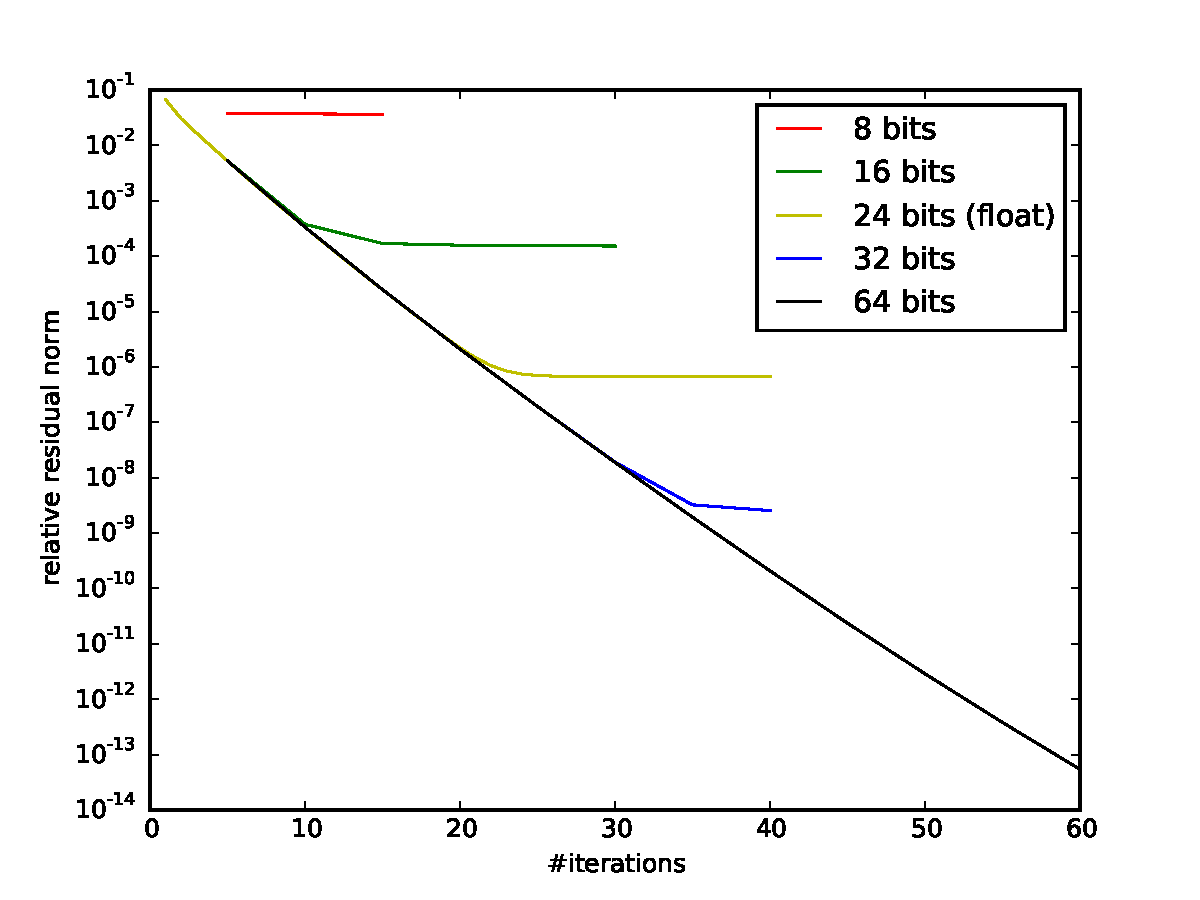
\includegraphics[width=0.8\linewidth]{figs/bits_convergence.pdf}
    \caption{Accuracy achievable with different number of bits in mantissa. Points (except for 24 bits) were obtained only for multiples of 5 iterations, but it is enough to see the thresholds appear.}
    \label{fig.bits_accuracy}
   \end{figure}
   
   The second thing to see is that \emph{AMGfloat} behaves exactly as what we would expect from \emph{AMGmpfr(24)} (same accuracy as versions with more precision in the beginning, then it reaches a threshold between that of \emph{AMGmpfr(16)} and that of \emph{AMGmpfr(32)}) in terms of accuracy whereas more variables were changed from \texttt{double} to \texttt{float}. It does not degrade more the accuracy, only a few variables
   from the 8 scalars actually control the final precision as they are temporary variables used for intermediate computations before being plugged back into the input matrix/vector.
   That being said, we design a new algorithm that adapts the precision of the variables during the execution. It is the same algorithm as \emph{AMGmpfr(b)} except this time the precision can change between two cycles.
   We fix a threshold on the ratio between the relative residual norm at two consecutive steps to trigger the precision change.
   Figure~\ref{fig.prec_incr} presents the evolution of accuracy for the original algorithm, 3 different strategies with increasing precision and a threshold of 0.8: start at $b=16$ and do $b=b+8$, start at $b=32$
   and do $b=b+8$, and start at $b=16$ and do $b=b\times2$. We run these strategies on a 240x240x240 matrix size with a 3x3x3 topology for \textsc{3DLaplace-27pt}.
   
   \begin{figure} \centering
    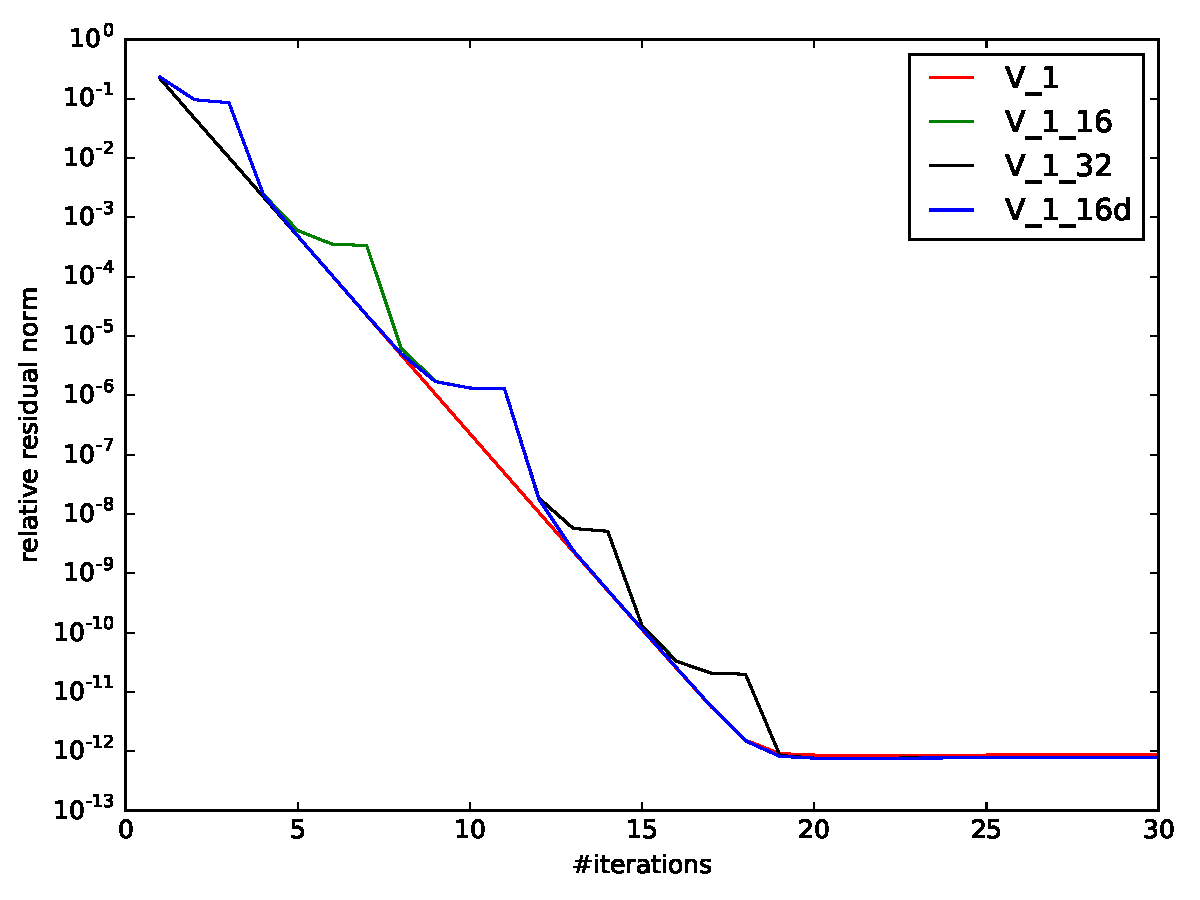
\includegraphics[width=0.8\linewidth]{figs/prec_incr.pdf}
    \caption{Accuracy of adaptive algorithms compared to the original double-precision with a threshold for updating the precision of $0.8$.}
    \label{fig.prec_incr}
   \end{figure}
   
   We see some steps appear, corresponding to the lower bound on the accuracy at the current precision. Then the precision is adapted to be able to improve the overall accuracy. Even if we lose some accuracy by waiting for the ratio
   between two consecutive relative residual norm to be higher than the threshold, when the precision changes, the convergence rate is more important (for one cycle) than that of the original algorithm (i.e. the slope is bigger on the figure), which makes any of
   the 3 versions able to reach the maximum accuracy (of $4.7\times 10^{-13}$) in the same number of cycles as the original algorithm (20-21 cycles).
   
   Two questions arise at this step. How to evaluate the energy/time savings of this adaptive algorithm? Which precisions should be used to optimize these savings?\\
   The first question is not simple because the use of the MPFR library to do these accuracy experiments introduce a huge overhead in the computations (running \emph{AMGmpfr(53)} is about 20 times longer than running \emph{AMG} whereas it
   represents the final same algorithm), and this overhead is not highly influenced by the choice of the number of bits. Thus it is impossible just to measure the execution time of the algorithm using MFPR library.
